\documentclass[11pt]{article}

\usepackage{enumitem}
\usepackage{natbib}
\usepackage{bibentry}
\usepackage{amssymb}
\usepackage{amsmath}
\usepackage{appendix}
\usepackage[margin=1in, paperwidth=8.5in, paperheight=11in]{geometry}
\usepackage[colorlinks=true,linkcolor=blue,citecolor=blue,urlcolor=blue]{hyperref}
\usepackage{fancyhdr}
\usepackage{wrapfig}
\usepackage{graphicx}

%\setlength{\parindent}{0in}

%% \usepackage{titlesec}
%% \titleformat*{\section}{\Large\scshape}
%% \titleformat*{\subsection}{\large}
%% \titleformat*{\subsubsection}{\large}

\setcounter{tocdepth}{2}

\pagestyle{fancy}
\lhead{\footnotesize Large-eddy Simulation Code Documentation}
\rhead{\footnotesize Page $|$ \thepage}
\cfoot{}

\begin{document}

\begin{titlepage}
\begin{center}

\vspace*{4cm}

\textsc{\LARGE \bf Large-Eddy Simulation Code Documentation}\\
[3cm]

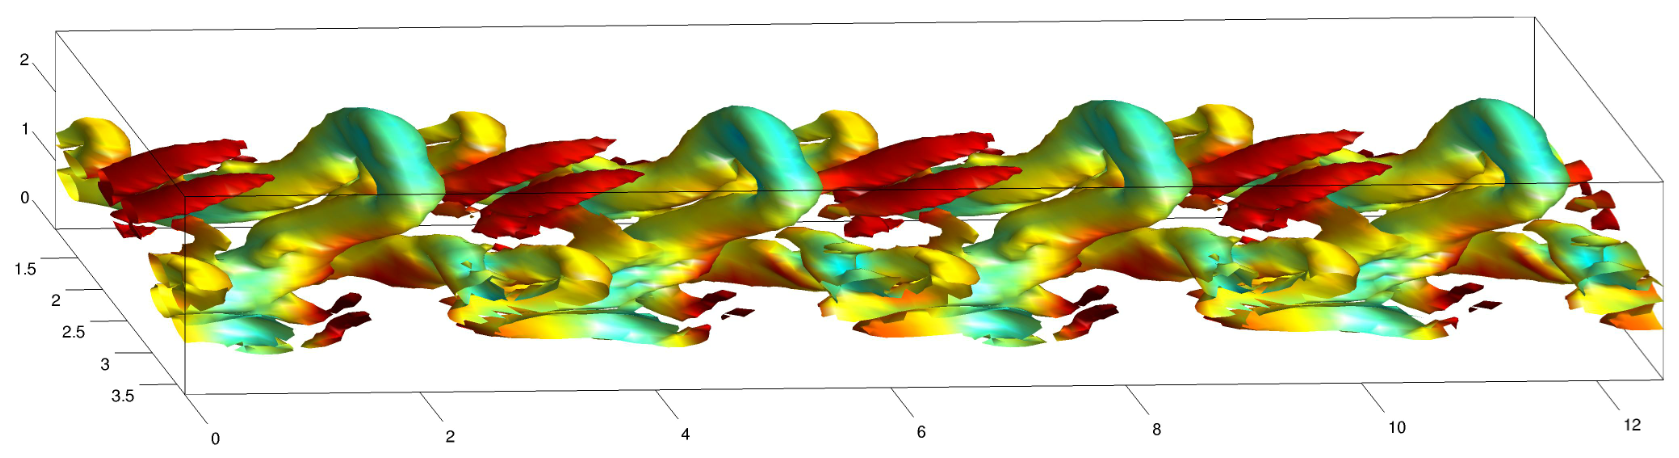
\includegraphics[width=\textwidth]{graphics/structures.png}

\vspace{5.5cm}

\begin{center}

\includegraphics[width=2.5cm]{graphics/UofU_Seal.pdf}
\end{center}

\textsc{\Large University of Utah} \\
Department of Mechanical Engineering \\

\end{center}

\end{titlepage}

\tableofcontents

\newpage

\section{Directory Structure}

\subsection{bin} Executables generated from compiling the code are placed here (see \S \ref{compiling}).

\subsection{checkpoints} Simulation checkpoint files (*.break) are written here.  This directory also contains an ASCII text file `break' that is used to log checkpointing information.

\subsection{input} Code input files (*.ini) are kept here.  This directory also contains an ASCII text file `LESinputs.txt', which gives (scalar) input parameters for the simulation.

\subsection{output}

\subsection{samples}

\subsection{src}

\subsection{utilities}(see \S \ref{utilities}).


\newpage
\section{Compiling}\label{compiling}

\newpage
\section{Simulation Inputs}\label{simulation_inputs}

\subsection{LESinputs.txt}

\subsection{binary input files}

\newpage
\section{Running the Simulation}\label{running_the_simulation}

\newpage
\section{Sample Cases}\label{sample_cases}

\newpage
\section{Utilities}\label{utilities}

\subsection{calc\_hprocs}

\clearpage

\bibliographystyle{apalike}
\bibliography{Master_Ref}

\end{document}
